\documentclass{beamer}

% \usepackage{beamerthemesplit} // Activate for custom appearance

\usepackage{listings}
\usepackage{graphicx}
\usepackage{minted}
\usepackage{hyperref}
\hypersetup{colorlinks=true}
\lstnewenvironment{code}{\lstset{language=Python,basicstyle=\small}}{}

\title{Z3 and Me}
\author{Chad Brewbaker\\ DataCulture LLC}
\date{May 23, 2016}

\begin{document}

\frame{\titlepage}


\begin{frame}[fragile]
Z3 is an open source SMT solver released by Microsoft.\\
SMT = Satisfiability Modulo Theories\\
\\
Boolean logic (True, False, And, Or, Not) +\\
Theories: empty theory, linear arithmetic, nonlinear arithmetic, bitvectors, arrays, datatypes, and quantifiers
\end{frame}


\begin{frame}[fragile]
Why would I want to use a SMT solver?\\
\\
Solve logic problems.\\
Optimize processes.\\
Prove correctness.\\
\end{frame}

\begin{frame}[fragile]
%Silly Facebook Problem

\includegraphics[scale=0.5]{spuzzle}
\end{frame}

\begin{frame}[fragile]
\inputminted{Python}{silly.py}
\input{silly.out}
\end{frame}


\begin{frame}[fragile]
SAT/SMT Solver Performance over time\\\\
1998 1,000 contraints\\\\
2001 10,000 constraints\\\\
2005 100,000 constraints\\\\
2010 1,000,000 constraints\\\\
(Data by Vijay Ganesh)
\end{frame}


\begin{frame}[fragile]
``Control-flow hijacking vulnerabilities represent more than 50\% of all vulnerabilities reported." - Oliveira 2016
\includegraphics[scale=0.3]{dragon}
\\``Rainbow Books scene", Hackers, United Artists, 1995
\end{frame}

\begin{frame}[fragile]
Microsoft SAGE Fuzzer
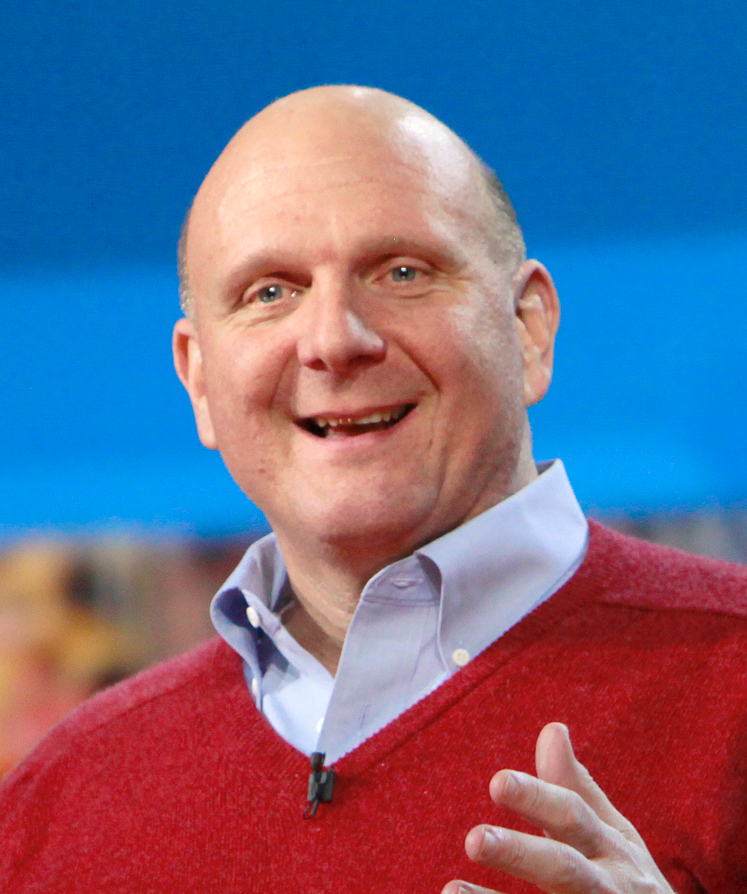
\includegraphics[scale=0.5]{sage}\\
Built on Z3. \\ Proprietary. \\Found ${1\over 3}$ bugs in Windows 7-10.
\end{frame}

\begin{frame}[fragile]
Symbolic + Concrete = Concolic testing\newline
\newline\newline Compile with code coverage. 
\newline\newline Find untouched code branches.
\newline\newline Use SMT solver find assignment of variables that allows branch to be entered.
\end{frame}

\begin{frame}[fragile]
Concolic testing example:\newline\newline
Fizz Buzz Jaberwocky
\end{frame}

\begin{frame}[fragile]
\inputminted{Python}{jabberwocky.py}
\input{jabberwocky.out}
\end{frame}


\begin{frame}[fragile]
American Fuzzy Lop
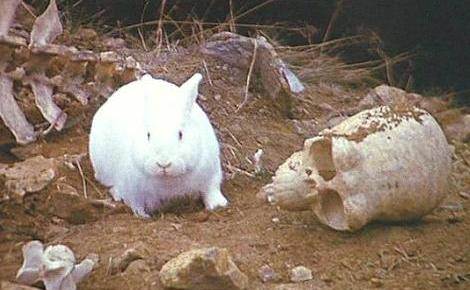
\includegraphics[scale=0.5]{killerRabbit}
\newline\url{https://fuzzing-project.org/}
\newline ImageTragick, Shellshock, PHP, OpenSSL, Mozilla, SQLlite, ...
\end{frame}

\begin{frame}[fragile]
American Fuzzy Lop demo on stock OSX.
\end{frame}


\begin{frame}[fragile]
Systems data one liners.\\
How do we inspect assembler calls?\\
How do we inspect raw operating system calls?\\
How do we inspect network calls?\\
\end{frame}

\begin{frame}[fragile]
Spying on C builds.\\
make VERBOSE=1 (Cmake)\\ 
make V=1 (GNU autotools)
\end{frame}

\begin{frame}[fragile]
clang -Os -S -emit-llvm sample.c -o sample.ll\newline\newline
llc -O3 sample.ll -march=x86 -o sample-x86.s\newline\newline
llc -O3 sample.ll -march=arm -o sample-arm.s
\end{frame}

\begin{frame}[fragile]
Spying on system calls.\\
strace (Linux)\\ 
dtrace (OS X)
\end{frame}

\begin{frame}[fragile]
Spying on network calls.\newline\newline
sudo tcpdump -i en0
\end{frame}

\begin{frame}
Use functional tools for your platform.\newline\newline
C++ $\rightarrow$ (Haskell, Elixir OTP)\newline\newline
Java VM $\rightarrow$ (Scala, Frege)\newline\newline
Javascript $\rightarrow$ (Elm, Typescript)
\end{frame}

\begin{frame}
Hopper,  formally specify multi-party contracts\newline\newline
Don't let contract attorneys hand waive. Prove coorectness.\newline\newline
Don't let contract attorneys waste executive manpower. Automate transactions.\newline\newline
https://github.com/hopper-lang/hopper
\end{frame}

\begin{frame}
1) Formal parsers on all inputs.\newline\newline
2) Isolate pure code from IO code.\newline\newline
3) Make the compiler do more work, not the tester.\newline\newline
4) Runtime monitoring with strace on vendor code.\newline\newline
5) Decouple monoliths.\newline\newline
6) Use Packer to maintain all dependencies. No black boxes.
\end{frame}

\begin{frame}
http://leanprover.github.io\newline\newline
http://z3prover.github.io\newline\newline
http://www.sympy.org/en/index.html\newline\newline
http://saw.galois.com\newline\newline
http://leventerkok.github.io/sbv/
\end{frame}

\begin{frame}
Girard (1987), Linear Logic\newline
Tinelli (2006), The Satisfiability Modulo Theories Library\newline
Ganesh (2007), Decision Procedures for Bit-Vectors, Arrays and Integers\newline
Lezama (2008), Program synthesis by sketching\newline
De Moura (2008), Z3: An efficient SMT solver\newline
Brummayer (2009), Fuzzing and delta-debugging SMT solvers\newline
Jovanovic (2015) Analysis and Design of Symmetric Cryptographic Algorithms 
\end{frame}


%Package depencency problem

% Verify optimization (powers of two)

% Knights problem



% Code coverage python

%Fizz, buzz, jaberwocky

% SAW

% AFL Fuzz




%\frame
%{
%  \frametitle{Features of the Beamer Class}
%
%  \begin{itemize}
%  \item<1-> Normal LaTeX class.
%  \item<2-> Easy overlays.
%  \item<3-> No external programs needed.      
%  \end{itemize}
%}
\end{document}

